\section{FRONTEND}\label{ch:frontend}

Das Frontend wurde mithilfe des Admin-Dashboard ngx-admin auf Basis von Angular 9+ und Nebular entwickelt. Mittels Angular wird eine Weboberfläche komponentenbasiert zur Verfügung gestellt. Für die serverseitige Anwendung benötigt Angular zudem Node.js, eine JavaScript-Laufzeitumgebung. Zudem wird ngx-admin mit dem Eva Design System unterstützt, um UI-Design zu vereinfachen. 

\subsection{Architektur}

In der unteren Abbildung (Fig. 2.) ist die Architektur des Frontend zu sehen. Eine Komponente besteht aus einem Template (HTML-Datei) und einem Style (SCSS-Datei). Diese werden als Metadaten im Dekorator der Komponente festgelegt und stellen die Ansicht dar. Mithilfe der Datenbindung kann das Template mit der Komponente Daten austauschen und gegebenenfalls Events ausführen. Bei Bedarf können Komponenten durch die Dependency Injection Zugriff auf eine Serviceklasse erhalten. Somit können wiederverwendbare Funktionen oder Daten aus dem Backend zur Verfügung gestellt werden. In den Modulen werden Komponenten, Module, Services usw. gruppiert und verwaltet. In Angular werden zwei Modularten unterschieden. Jedes Angular Projekt besitzt ein Root-Modul, das app.module.ts heißt. Diese ist dazu da, um die gesamte Webanwendung zu verwalten und diese wird beim Start der Anwendung als erstes geladen und initialisiert. Mit Feature-Modulen kann der Code, der sich auf eine bestimmte Funktionalität oder ein bestimmtes Feature bezieht, von anderem Code getrennt werden und bleibt somit organisiert.

\begin{figure}[thpb]
      \centering
      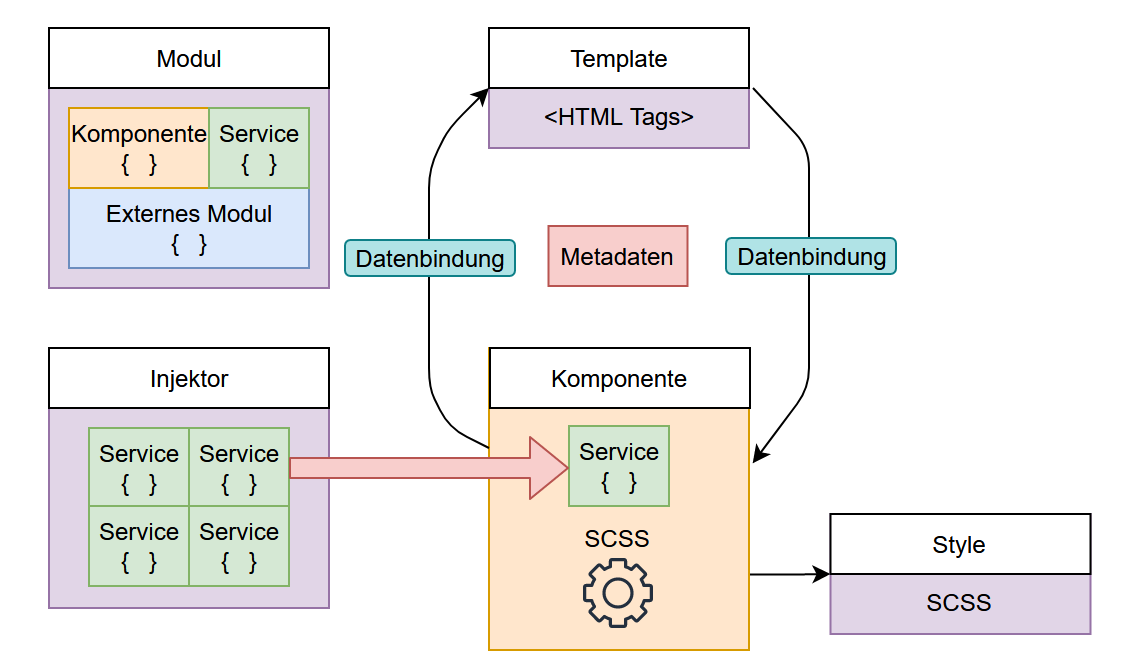
\includegraphics[scale=0.55]{abbildungen/frontend_architecture.png}
      \caption{Angular Architektur des Projektes}
      \label{fig:frontend}
 \end{figure}


\subsection{Entwickelte Komponenten}
Zusätzlich zu den vorhandenen Komponenten vom ngx-admin wurden folgende weitere Komponenten entwickelt (siehe TABLE 1).

\hyphenation{Komponenten}
\renewcommand{\arraystretch}{2}
\begin{table}[ht!]
  \centering
  \begin{tabular}{|c|p{4.4cm}|}
	\hline
	AirQualityChart & Bildet die Werte des Luftqualitätssensors in einem Liniendiagramm wieder. \\
	\hline
	AirQuality & Visualisiert die Werte des Luftqualitätssensors unter Verwendung der AirQualityChart Komponente. \\
	\hline
	buzzer-frequenzy & Ein Eingabefeld zum festsetzen der Frequenz des Piezoelements. \\
	\hline
	gant & Das Gantt-Diagramm zeigt an, ob jemand im Raum anwesend war oder nicht. \\
	\hline
    lcd-input & Ein Eingabefeld zum festsetzen des LCD-Displays auf dem Sensorknoten. \\
	\hline
	lineChartComponent & Ein universell verwendbares Liniendiagramm. \\
	\hline
	switch & Ein Knopf, der an- und ausgeschaltet werden kann. \\
	\hline
	temperatureGauge & Ein Tachometer zum visualisieren von verschiedenen Werten. \\
	\hline
	tempSensorCard & Kombination aus dem LineChartComponent und dem temperatureGauge Komponente. Stellt eine zweiseitige Karte dar, die auf der einen Seite Luftdruck, Luftfeuchtigkeit und Temperatur in einem Liniendiagramm darstellt und auf der anderen Seite ein Tachometer mit den aktuellen Werten. \\
	\hline
	sensornode-dashbord & In dieser Komponente werden die oben genannten Komponenten des jeweiligen Sensorknotens dargestellt. \\
	\hline
	led-display & Zeigt die LED-Anzeige des aktuellen Knotens. \\
	\hline
	Header (modifiziert) & Der vorhandene Header wurde modifiziert, um eine Zeitspanne auswählen zu können. \\
	\hline
  \end{tabular}
  \caption{Komponenten}
  \label{tab:beispiel}
\end{table}

\subsection{Entwickelte Services}

\hyphenation{Services}
\renewcommand{\arraystretch}{2}
\begin{table}[ht!]
  \centering
  \begin{tabular}{|c|p{4.4cm}|}
	\hline
	BackendDataService & Ist für die Kommunikation mit dem Backend zuständig. Zum Abfragen und Senden von Daten. \\
	\hline
	DashboardFunctionalityService & Auslagerung der Funktionen für die sensornode-dashboard Komponente. \\
	\hline
	SharedDataService & Stellt allen Komponenten ein Observable des ausgewählten Zeitraums und der aktuellen Sensorknoten-ID zur Verfügung. \\
	\hline
  \end{tabular}
  \caption{Services}
  \label{tab:beispiel}
\end{table}

\subsection{Routing}
Alle Verfügbaren seiten im Projekt repräsentieren ein Dashboard eines Sensorknotens.
Zugänglich sind diese über die URL: /pages/{Knoten-ID}. Siehe Listing 5.
\begin{lstlisting}[caption={Knoten-ID Routing},captionpos=b,showstringspaces=false, basicstyle=\small,label={lst:sensor_dtype}]
    {
      path: ':id',
      component: SensorNodeDashboardComponent
    }
\end{lstlisting}
Alle verfügbaren Knoten werden am Anfang aus dem Backend abgerufen, und anschließend links im Navigator als Menüpunkt angezeigt. Auf dem Dashboard des einzelnen Knotens werden über die aktuelle Knoten-ID die Anfragen an das Backend gesendet.